% change according to folder and file names
\ifpdf
    \graphicspath{{4/figures/PNG/}{4/figures/PDF/}{3/figures/}}
\else
    \graphicspath{{4/figures/EPS/}{4/figures/}}
\fi

%: ----------------------- contents from here ------------------------
\chapter{ΕΑ και ΜΑΕΑ Υποβοηθούμενοι από Ανάλυση Κυρίων Συνιστωσών } % top level followed by section, subsection
\label{VarCorrChapter}
%\begin{flushright}
%Any intelligent fool can make things  
%\linebreak
%bigger, more complex, and more violent. 
%\linebreak
%It takes a touch of genius, and a lot of  
%\linebreak
%courage, to move in the opposite direction.
%\linebreak
%Albert Einstein
%\end{flushright}
Το κεφάλαιο αυτό παρουσιάζει τρόπους με τους οποίους μπορεί να μειωθεί σημαντικά ο χρόνος βελτιστοποίησης με χρήση ΕΑ ή  παραλλαγών αυτών και, μάλιστα, υπερθετικά στη μείωση που επιφέρουν διάφοροι άλλοι ήδη γνωστοί τρόποι, όπως λ.χ. η προσεγγιστική προ-αξιολόγηση με μεταπρότυπα, κτλ.. Οι προτεινόμενοι τρόποι ενδείκνυνται για προβλήματα με μεγάλο αριθμό μεταβλητών σχεδιασμού και συνάρτηση κόστους $\Phi$ που είναι μη-διαχωρίσιμη (και ανισότροπη) ως προς τις μεταβλητές σχεδιασμού \cite{Salomon,Roy_2002a,Ghisu_2010}. Τα προβλήματα αυτά θα αναφέρονται ως «κακώς-τοποθετημένα» και προκαλούν μεγάλη καθυστέρηση στο ρυθμό σύγκλισης των ΕΑ ή των ΜΑΕΑ.  

Τα «κακώς-τοποθετημένα» προβλήματα έχουν σχέση με τον τρόπο που οι μεταβλητές σχεδιασμού ενός προβλήματος συσχετίζονται με συνάρτηση κόστους $\Phi$. Συνυφασμένες άμεσα με το πρόβλημα είναι οι έννοιες της ισότροπης ή μη-ισότροπης επίδρασης των μεταβολών τιμής των μεταβλητών σχεδιασμού στη μεταβολή τιμής της $\Phi$ και, κυρίως, του διαχωρίσιμου της. Η διαχείριση μιας μη-διαχωρίσιμης, μη-ισότροπης συνάρτησης-στόχου $\Phi$ κάνει το πρόβλημα βελτιστοποίησης «κακώς-τοποθετημένο». Τα μεγάλης διάστασης ($N»$) «κακώς-τοποθετημένα» προβλήματα βελτιστοποίησης χαρακτηρίζονται από μεγάλο κόστος επίλυσης μέσω των ΕΑ αλλά, ακόμη, και των ΜΑΕΑ. Επειδή δε τα περισσότερα βιομηχανικά προβλήματα ανήκουν σε αυτήν την κατηγορία, η επιθυμία για μείωση του κόστους επίλυσής τους είναι τεράστια.  Οι έννοιες της ισοτροπίας και του διαχωρίσιμου, καθώς και η επίδρασή τους στους ΕΑ, αναλύονται στην επόμενη ενότητα αυτού του κεφαλαίου. Από μαθηματικής σκοπιάς, ο εντοπισμός του τρόπου συσχέτισης της $\Phi$ με τις μεταβλητές σχεδιασμού υλοποιείται με την Ανάλυση σε Κύριες Συνιστώσες (ΑσΚΣ, \english{Principal Component Analysis \greek{ή} PCA}) \cite{Haykin}. Το κόστος χρήσης της ΑσΚΣ για τους σκοπούς του κεφαλαίου αυτού είναι το κόστος επίλυσης ιδιοπροβλημάτων μικρής διάστασης και κρίνεται, ως εκ τούτου, πάρα πολύ μικρό. Γίνεται, μάλιστα, αμελητέο όταν ο ΕΑ ή ο ΜΑΕΑ χρησιμοποιεί υψηλού κόστους λογισμικό αξιολόγησης των υποψήφιων λύσεων, όπως λ.χ. κώδικες ΥΡΔ.

Το κεφάλαιο αυτό προτείνει και πιστοποιεί, ως προς την αποδοτικότητα τους, δύο τρόπους εκμετάλλευσης των συσχετίσεων των μεταβλητών σχεδιασμού (ως προς τη $\Phi$) που εντοπίζει η ΑσΚΣ ή \english{PCA}. Ο πρώτος τρόπος σχετίζεται με την τροποποίηση των εξελικτικών τελεστών και θα αναφέρεται ως ΕΑ(\english{PCA}) ή ΜΑΕΑ(\english{PCA}) \cite{LTT_2_054}. Ο δεύτερος τρόπος σχετίζεται με τη χρήση μεταπροτύπων στο ΜΑΕΑ. Συγκεκριμένα, χρησιμοποιεί την πληροφορία που παρέχει η ΑσΚΣ κατά την ΠΠΑ των υποψήφιων λύσεων με μεταπρότυπα, ώστε τα τελευταία να εκπαιδεύονται με μικρό αριθμό σημαντικών εισόδων. Η μείωση αυτή του πλήθους εισόδων των μεταπροτύπων αυξάνει την αξιοπιστία τους, επιτρέπει τη χρήση τους νωρίτερα στο ΜΑΕΑ και επιφέρει υπολογιστικό κέρδος. Ο δεύτερος αυτός τρόπος θα αναφέρεται ως Μ(\english{PCA})ΑΕΑ. Στο ακρωνύμιο αυτό, ο προσδιορισμός \english{PCA} τοποθετείται μετά το Μ (Μ=\english{metamodel}, μεταπρότυπο) για να φανεί ακριβώς το που χρησιμοποιείται. Προφανώς, οι δύο τρόποι μπορούν να χρησιμοποιηθούν συνδυαστικά, σε μια νέα μέθοδο που θα αποκαλείται Μ(\english{PCA})ΑΕΑ(\english{PCA}).

Στο δεύτερο τμήμα του κεφαλαίου αυτού, οι προτεινόμενες τεχνικές πιστοποι-ούνται σε προβλήματα ελαχιστοποίησης κακώς-τοποθετημένων μαθηματικών συναρτήσεων. Στη συνέχεια, εκτίμηση του αναμενόμενου κέρδους γίνεται και σε ένα πρόβλημα σχεδιασμού-βελτιστοποίησης της μορφής της αεροτομής μιας 2Δ πτερύγωσης συμπιεστή. Βιομηχανικού ενδιαφέροντος εφαρμογές των προτεινόμενων μεθόδων παρουσιάζονται σε επόμενα κεφάλαια.             

 
%Σε αυτό το κεφάλαιο αρχικά παρουσιάζονται οι πιθανές ιδιαιτερότητες μιας συνάρτησης κόστους που ενδέχεται να προκαλέσουν συσχετίσεις μεταξύ των μεταβλητών σχεδιασμού (ΣΜΣ) \cite{Salomon,Roy_2002a,Ghisu_2010}. Στη συνέχεια, διερευνάται η επίδραση τους στους ΕΑ και αργότερα προτείνεται μία μέθοδος εντοπισμού αυτών των συσχετίσεων κάνονας χρήση Ανάλυσης σε Κύριες Συνιστώσες (ΑσΚΣ), \english{Principal Component Analysis (PCA)} και μέθοδοι αξιοποίησης τους αναβαθμίζοντας του τελεστές εξέλιξης. Προτείνεται, επίσης, η χρήση των ιδιοτιμών που υπολογίζονται από την ΑσΚΣ σαν μετρική σημαντικότητας των κατευθύνσεων στον χώρο σχεδιασμού και η αποκοπή των λιγότερο σημαντικών από αυτές κατά τη διαδικασία εκπαίδευσης του μεταπροτύπου.

%Τέλος οι προτεινόμενες τεχνικές πιστοποιούνται μέσα από αριθμό προβλημάτων μαθηματικής βελτιστοποίησης, ειδικά επιλεγμένων ούτως ώστε να εμπίπτουν στην κατηγορία των προβλημάτων με ΣΜΣ, και στον σχεδιασμό 2Δ πτερύγωσης συμπιεστή.
    
\section{Δυσκολίες λόγω Ιδιαιτερότητας της Συνάρτησης Κόστους}
Ένα πρόβλημα βελτιστοποίησης αναφέρεται ως «κακώς τοποθετημένο» αν παρουσιάζει συνδυασμό δύο ιδιαιτεροτήτων της συνάρτησης-κόστους $\Phi$ (σχήμα \ref{nonsep}): α) τη μη-ισότροπη συνεισφορά των μεταβλητών σχεδιασμού στη συνάρτηση κόστους και β) το μη-διαχωρίσιμο της $\Phi$.

Μη-ισότροπη συνεισφορά των μεταβλητών σχεδιασμού στη συνάρτηση-κόστους υπάρχει όταν ισόποσες μεταβολές των μεταβλητών σχεδιασμού δεν επιφέρουν ισόποσες μεταβολές στην τιμή της $\Phi$.  Μια συνάρτηση κόστους $\Phi$ ονομάζεται διαχωρίσιμη ως προς τη μεταβλητή σχεδιασμού $x_i$ αν η βέλτιστη τιμή του $x_i$ είναι ανεξάρτητη των τιμών των υπολοίπων μεταβλητών σχεδιασμού. Η $\Phi$ ονομάζεται διαχωρίσιμη αν είναι διαχωρίσιμη ως προς όλες τις μεταβλητές σχεδιασμού.        

\begin{figure}[h!]
\begin{minipage}[b]{1\linewidth}
 \centering
 \resizebox*{14cm}{!}{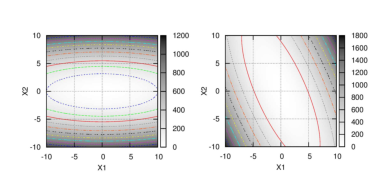
\includegraphics{ellipseB.eps}}
\end{minipage}
%\begin{minipage}[b]{0.45\linewidth}
% \centering
% \resizebox*{9cm}{!}{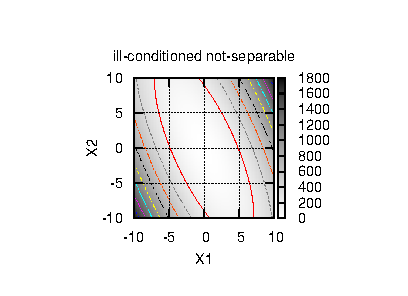
\includegraphics{ellipseturn.eps}}
%\end{minipage}
\caption{Πρόβλημα βελτιστοποίησης με μη-ισότροπη συνεισφορά των μεταβλητών σχεδιασμού στην $f$ (αριστερά). Πρόκειται για ισοϋψείς της $f$ της σχέσης \ref{ellipse} για Ν=2. Η μεταβλητή $x_2$ συνεισφέρει σε μεγαλύτερο βαθμό στην $f$ από ότι η $x_1$. Από την άλλη πλευρά, η $f$ είναι διαχωρίσιμη, άρα το πρόβλημα, ουσιαστικά δεν είναι «κακώς τοποθετημένο». Πρόβλημα βελτιστοποίησης με μη-ισότροπη συνεισφορά των μεταβλητών σχεδιασμού και μη-διαχωρίσιμες μεταβλητές σχεδιασμού ως προς την $f$ (δεξιά). Πρόκειται για ισοϋψείς της $f$ της σχέσης \ref{ellipse2} για Ν=2. Η βέλτιστη τιμή της $x_1$ εξαρτάται πλέον από τη $x_2$ και αντιστρόφως. Άρα, το πρόβλημα βελτιστοποίησης είναι πλέον «κακώς τοποθετημένο», κάτι που θα φανεί ιδιαίτερα λύνοντας το για μεγάλες τιμές του Ν.} 
\label{nonsep}
\end{figure}

Η επίδραση των παραπάνω χαρακτηριστικών στη συνάρτηση-στόχου $f$ σε ένα πρόβλημα βελτιστοποίησης, όταν αυτό επιλύεται με ΕΑ,  διερευνάται μέσω δύο προβλημάτων μαθηματικής βελτιστοποίησης επιλεγμένων ώστε να εμπίπτουν σε αυτήν την κατηγορία. Σκοπός της διερεύνησης είναι να δειχθεί ότι, αν το ίδιο πρόβλημα βελτιστοποίησης επαναδιατυπωθεί ως προς νέες μεταβλητές σχεδιασμού, ίδιου πλήθους, ως προς τις οποίες η υπόψη συνάρτηση κόστους είναι πλέον διαχωρίσιμη, ο ΕΑ εντοπίζει τη βέλτιστη λύση σε πολύ μικρότερο αριθμό αξιολογήσεων.  

Το πρώτο πρόβλημα αφορά ελαχιστοποίηση ενός πολυδιάστατου ελλειψοειδούς (η 2Δ μορφή του παρουσιάζεται στο σχήμα \ref{nonsep}). Η διαχωρίσιμη μορφή του περιγράφεται από τη σχέση   

\begin{eqnarray}
   \Phi=f(\vec{x})=\sum^{N}_{i=1}a^{\frac{i-1}{N-1}}x_i^2
   \label{ellipse} 
\end{eqnarray}
όπου $a$ είναι, πρακτικά, ο ο αριθμός κατάστασης της συνάρτησης. Μεγάλες τιμές της ποσότητας $a$ $(a>>1)$ ενισχύουν τη μη-ισότροπη συνεισφορά των μεταβλητών σχεδιασμού στην $f$.

Εναλλακτικά, μια μη-διαχωρίσιμη μορφή του ίδιου προβλήματος μπορεί να διατυπωθεί ως 
\begin{eqnarray}
   \Phi=f(\vec{x})=\sum^{N}_{i=1}a^{\frac{i-1}{N-1}}y_i^2
   \label{ellipse2} 
\end{eqnarray}
όπου $\vec{y}=B\vec{x}$ και $B$ ένα ($N\times N$) μητρώο στροφής. Η σύγκριση των σχέσεων \ref{ellipse} και \ref{ellipse2} φαίνεται εποπτικά, για Ν=2, στο σχήμα \ref{nonsep}. Ουσιαστικά, οι σχέσεις \ref{ellipse} και \ref{ellipse2} αναφέρονται στο ίδιο πρόβλημα ελαχιστοποίησης, με τη μορφή \ref{ellipse} να πλεονεκτεί της \ref{ellipse2} όταν η επίλυση γίνεται με ΕΑ ή ΜΑΕΑ.  

Η δεύτερη περίπτωση μαθηματικής βελτιστοποίησης αφορά στην ελαχιστοποίηση της πολυτροπικής (με πολλά τοπικά ακρότατα) συνάρτησης 

\begin{eqnarray}
  \Phi=f(\vec{x})=10N+(\sum^{N}_{i=1}x_i)^2 - 10Ncos(\pi  \sum^{N}_{i=1}x_i)
   \label{mm} 
\end{eqnarray}

Η συνάρτηση \ref{mm} αποτελεί τη μη-διαχωρίσιμη εκδοχή του προβλήματος βελτιστοποίησης. Η αντίστοιχη διαχωρίσιμη εκδοχή υπάρχει και προκύπτει, όμοια με την περίπτωση του ελλειψοειδούς, αν το $\vec{x}$ αντικατασταθεί απο το $\vec{y}$ όπου $\vec{y}=B\vec{x}$ και $B$ κατάλληλο μητρώο στροφής. Η συνάρτηση \ref{mm}, έχοντας, στην πραγματικότητα, μόνο μια σημαντική κατεύθυνση στο χώρο σχεδιασμού ($\sum^{N}_{i=1}x_i$), ανήκει στην κατηγορία των συναρτήσεων με εξαιρετικά μη-ισότροπη συνεισφορά των μεταβλητών σχεδιασμού στην $f$ (ως εάν $a=\infty$ στο προηγούμενο παράδειγμα). 
%Αυτή είναι μια πολύ σημαντική κατηγορία προβλημάτων γιατί προσομοιάζει σε συμπεριφορά τα προβλήματα βελτιστοποίησης πολλών στόχων, όπου στην πραγματικότητα μια περιοχή του χώρου των λύσεων εμπεριέχει όλους τους βέλτιστους σχεδιασμούς.           

Συγκριτικές πορείες σύγκλισης μεταξύ διαχωρίσιμης και μη-διαχωρίσιμης εκδοχής του $30$Δ ($N\!=\!30$) ελλειψοειδούς και της συνάρτησης \ref{mm} παρουσιάζονται στο σχήμα \ref{ellipse_t2}. Οι πορείες σύγκλισης απεικονίζουν μέσες τιμές υπολογισμένες για $10$ διαφορετικά τρεξίματα ΕΑ, με διαφορετική αρχικοποίηση της γεννήτριας τυχαίων αριθμών.  Παρατηρείται ότι, και στις δύο περιπτώσεις η διαχωρίσιμη εκδοχή των προβλημάτων υπερτερεί σημαντικά σε ταχύτητα της μη-διαχωρίσιμης εκδοχής αυτών. Το κέρδος  είναι σημαντικά μεγαλύτερο στην περίπτωση όπου $a=\infty$.        

\begin{figure}[h!]
%\begin{minipage}[b]{0.5\linewidth}
% \centering
% \resizebox*{7.5cm}{!}{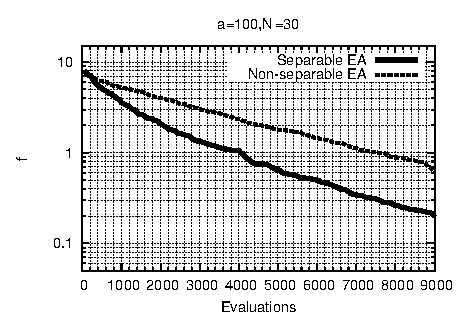
\includegraphics{100_30d.eps}}
%\end{minipage}
\begin{minipage}[b]{0.5\linewidth}
 \centering
 \resizebox*{7.5cm}{!}{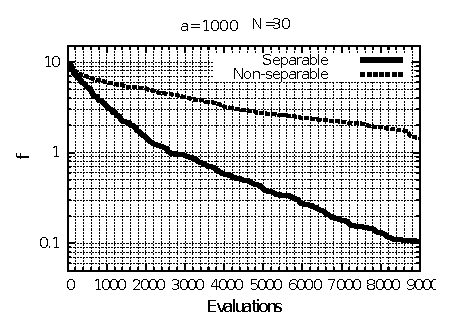
\includegraphics{1000_30db.eps}}
\end{minipage}
\begin{minipage}[b]{0.5\linewidth}
 \centering
 \resizebox*{7.5cm}{!}{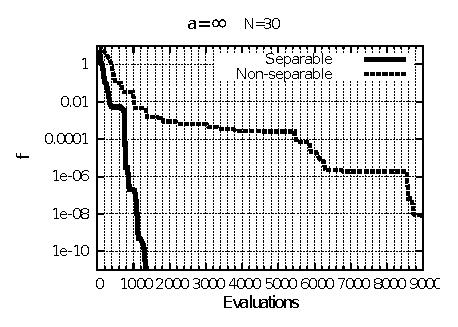
\includegraphics{30db.eps}}
\end{minipage}
\caption{Πορείες σύγκλισης ΕΑ για το 30Δ ελλειψοειδές με αριθμό κατάστασης (με $a=1000$) (αριστερά) και για την 30Δ συνάρτηση της σχέσης \ref{mm} (ως εάν $a=\infty$ στο προηγούμενο παράδειγμα) (δεξιά). Κάθε πρόβλημα λύνεται 10 φορές στη διαχωρίσιμη και άλλες 10 στη μη-διαχωρίσιμη εκδοχή του και σχεδιάζεται η μέση πορεία σύγκλισης κάθε εκδοχής.} 
\label{ellipse_t2}
\end{figure}



\section{Η Προτεινόμενη ΑσΚΣ}
Η προτεινόμενη μέθοδος κάνει χρήση της ΑσΚΣ για να υπολογίσει χρήσιμα τοπολογικά χαρακτηριστικά του συνόλου των επιλέκτων τα οποία και θεωρούνται αντιπροσωπευτικά των συσχετίσεων της $f$ ως προς τις μεταβλητές σχεδιασμού. Πιο αναλυτικά, αφού το σύνολο των επιλέκτων μετατραπεί σε ένα τυποποιημένο σύνολο δεδομένων Χ, \cite{Axler_1997}, δημιουργείται ο πίνακας συνδιακύμανσης $P_{N\times N}$ από τη σχέση 

\begin{equation} 
   P_{N\times N}= \frac{1}{e}XX^T
   \label{Cov_Mat} 
\end{equation}
όπου $e$ το πλήθος των επιλέκτων $P_e^g$ και $X$ ο πίνακας που έχει ως γραμμές τα διανύσματα σχεδιασμού που συνθέτουν το $P_e^g$ σε μορφή τυποποιημένου συνόλου δεδομένων.

Κάνοντας χρήση του φασματικού θεωρήματος αποσύνθεσης (\english{spectral decomposition theorem}),
 \cite{Axler_1997, Fodor_2002}, ο $P_{N\times N}$ μπορεί να γραφεί ως

\begin{equation} 
   P_{N\times N}= U\Lambda U^T
   \label{spectral}
\end{equation}
όπου $\Lambda\!=\!diag(\lambda_1 , . . . , \lambda_N )$ το διαγώνιο μητρώο των ιδιοτιμών και $U$ το $N\!\times\!N$ μητρώο των ιδιοδιανυσμάτων. 
Τα υπολογισθέντα ιδιοδιανύσματα (σχήμα \ref{reco1}) είναι οι κατευθύνσεις στο χώρο σχεδιασμού ως προς τις οποίες η $f$ είναι, κατά το δυνατό, διαχωρίσιμη. Αν ο ΕΑ χειριζόταν αγνώστους αναδιατυπωμένους σε αυτές τις κατευθύνσεις, το πρόβλημα βελτιστοποίησης θα μετατρεπόταν σε «λιγότερο  μη-διαχωρίσιμο» και, άρα, θα επιλυόταν με μικρότερο υπολογιστικό κόστος. Αυτήν την ιδέα υλοποιεί η προτεινόμενη μέθοδος.     

\begin{figure}[h!]
\begin{minipage}[b]{1\linewidth}
 \centering
 \resizebox*{!}{4.5 cm}{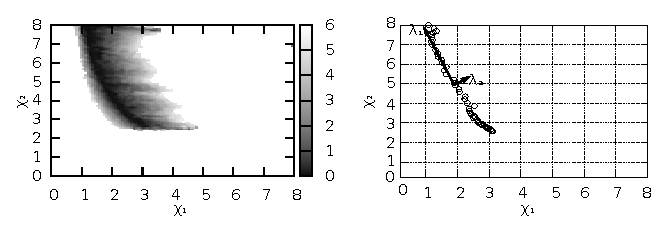
\includegraphics{DOFs.eps}}
\end{minipage}
\caption{Κατανομή της $f$ (ή της βαθμωτής $\Phi$ από λ.χ. τη διαδικασία \english{SPEA2}, για κάποια γενιά του ΕΑ, σε προβλήματα πολυκριτηριακής βελτιστοποίησης) στο χώρο σχεδιασμού (αριστερά). Το σύνολο των επίλεκτων $P^g_e$, για τη δεδομένη γενιά, και οι νέες κατευθύνσεις, στον χώρο σχεδιασμού,  $\lambda_1$ και $\lambda_2$, που ανέδειξε η ΑσΚΣ (αριστερά).} 
\label{reco1}
\end{figure}
       

\section{Εξελικτικοί Τελεστές Υποβοηθούμενοι από ΑσΚΣ} 

Με στόχο την επαναδιατύπωση του προβλήματος βελτιστοποίησης, χρησιμοποιώντας την πληροφορία που έδωσε  ΑσΚΣ για την υπόψη $f$, η παρούσα διατριβή προτείνει την εφαρμογή των τελεστών εξέλιξης (μετάλλαξης και διασταύρωσης), στο ευθυγραμμισμένο με τις νέες μεταβλητές σχεδιασμού που ανέδειξε η ΑσΚΣ. Με αυτήν την τακτική, η εξέλιξη λαμβάνει χώρα στο μετασχηματισμένο και κατά το δυνατό διαχωρίσιμο πρόβλημα βελτιστοποίησης, έχοντας σκοπό να ανακτήσει το (κατά το δυνατό) μεγαλύτερο ποσοστό απώλειας της απόδοσης του ΕΑ (σχήμα \ref{ellipse_t2}), που προκαλεί το μη-διαχωρισμό της $f$. Πληροφορίες σχετικές με τις ΣΜΣ προσδιορίζονται μέσω της ΑσΚΣ, η οποία επαναλαμβάνεται κάθε φορά που ένα νέο άτομο προστίθεται στο σύνολο των επιλέκτων. Η αξιοπιστία των υπολογιζόμενων ΣΜΣ ενισχύεται όσο το σύνολο των επιλέκτων προσεγγίζει το πραγματικό μέτωπο \english{Pareto}.              

%\begin{figure}[h!]
%\begin{minipage}[b]{1\linewidth}
% \centering
% \resizebox*{14cm}{!}{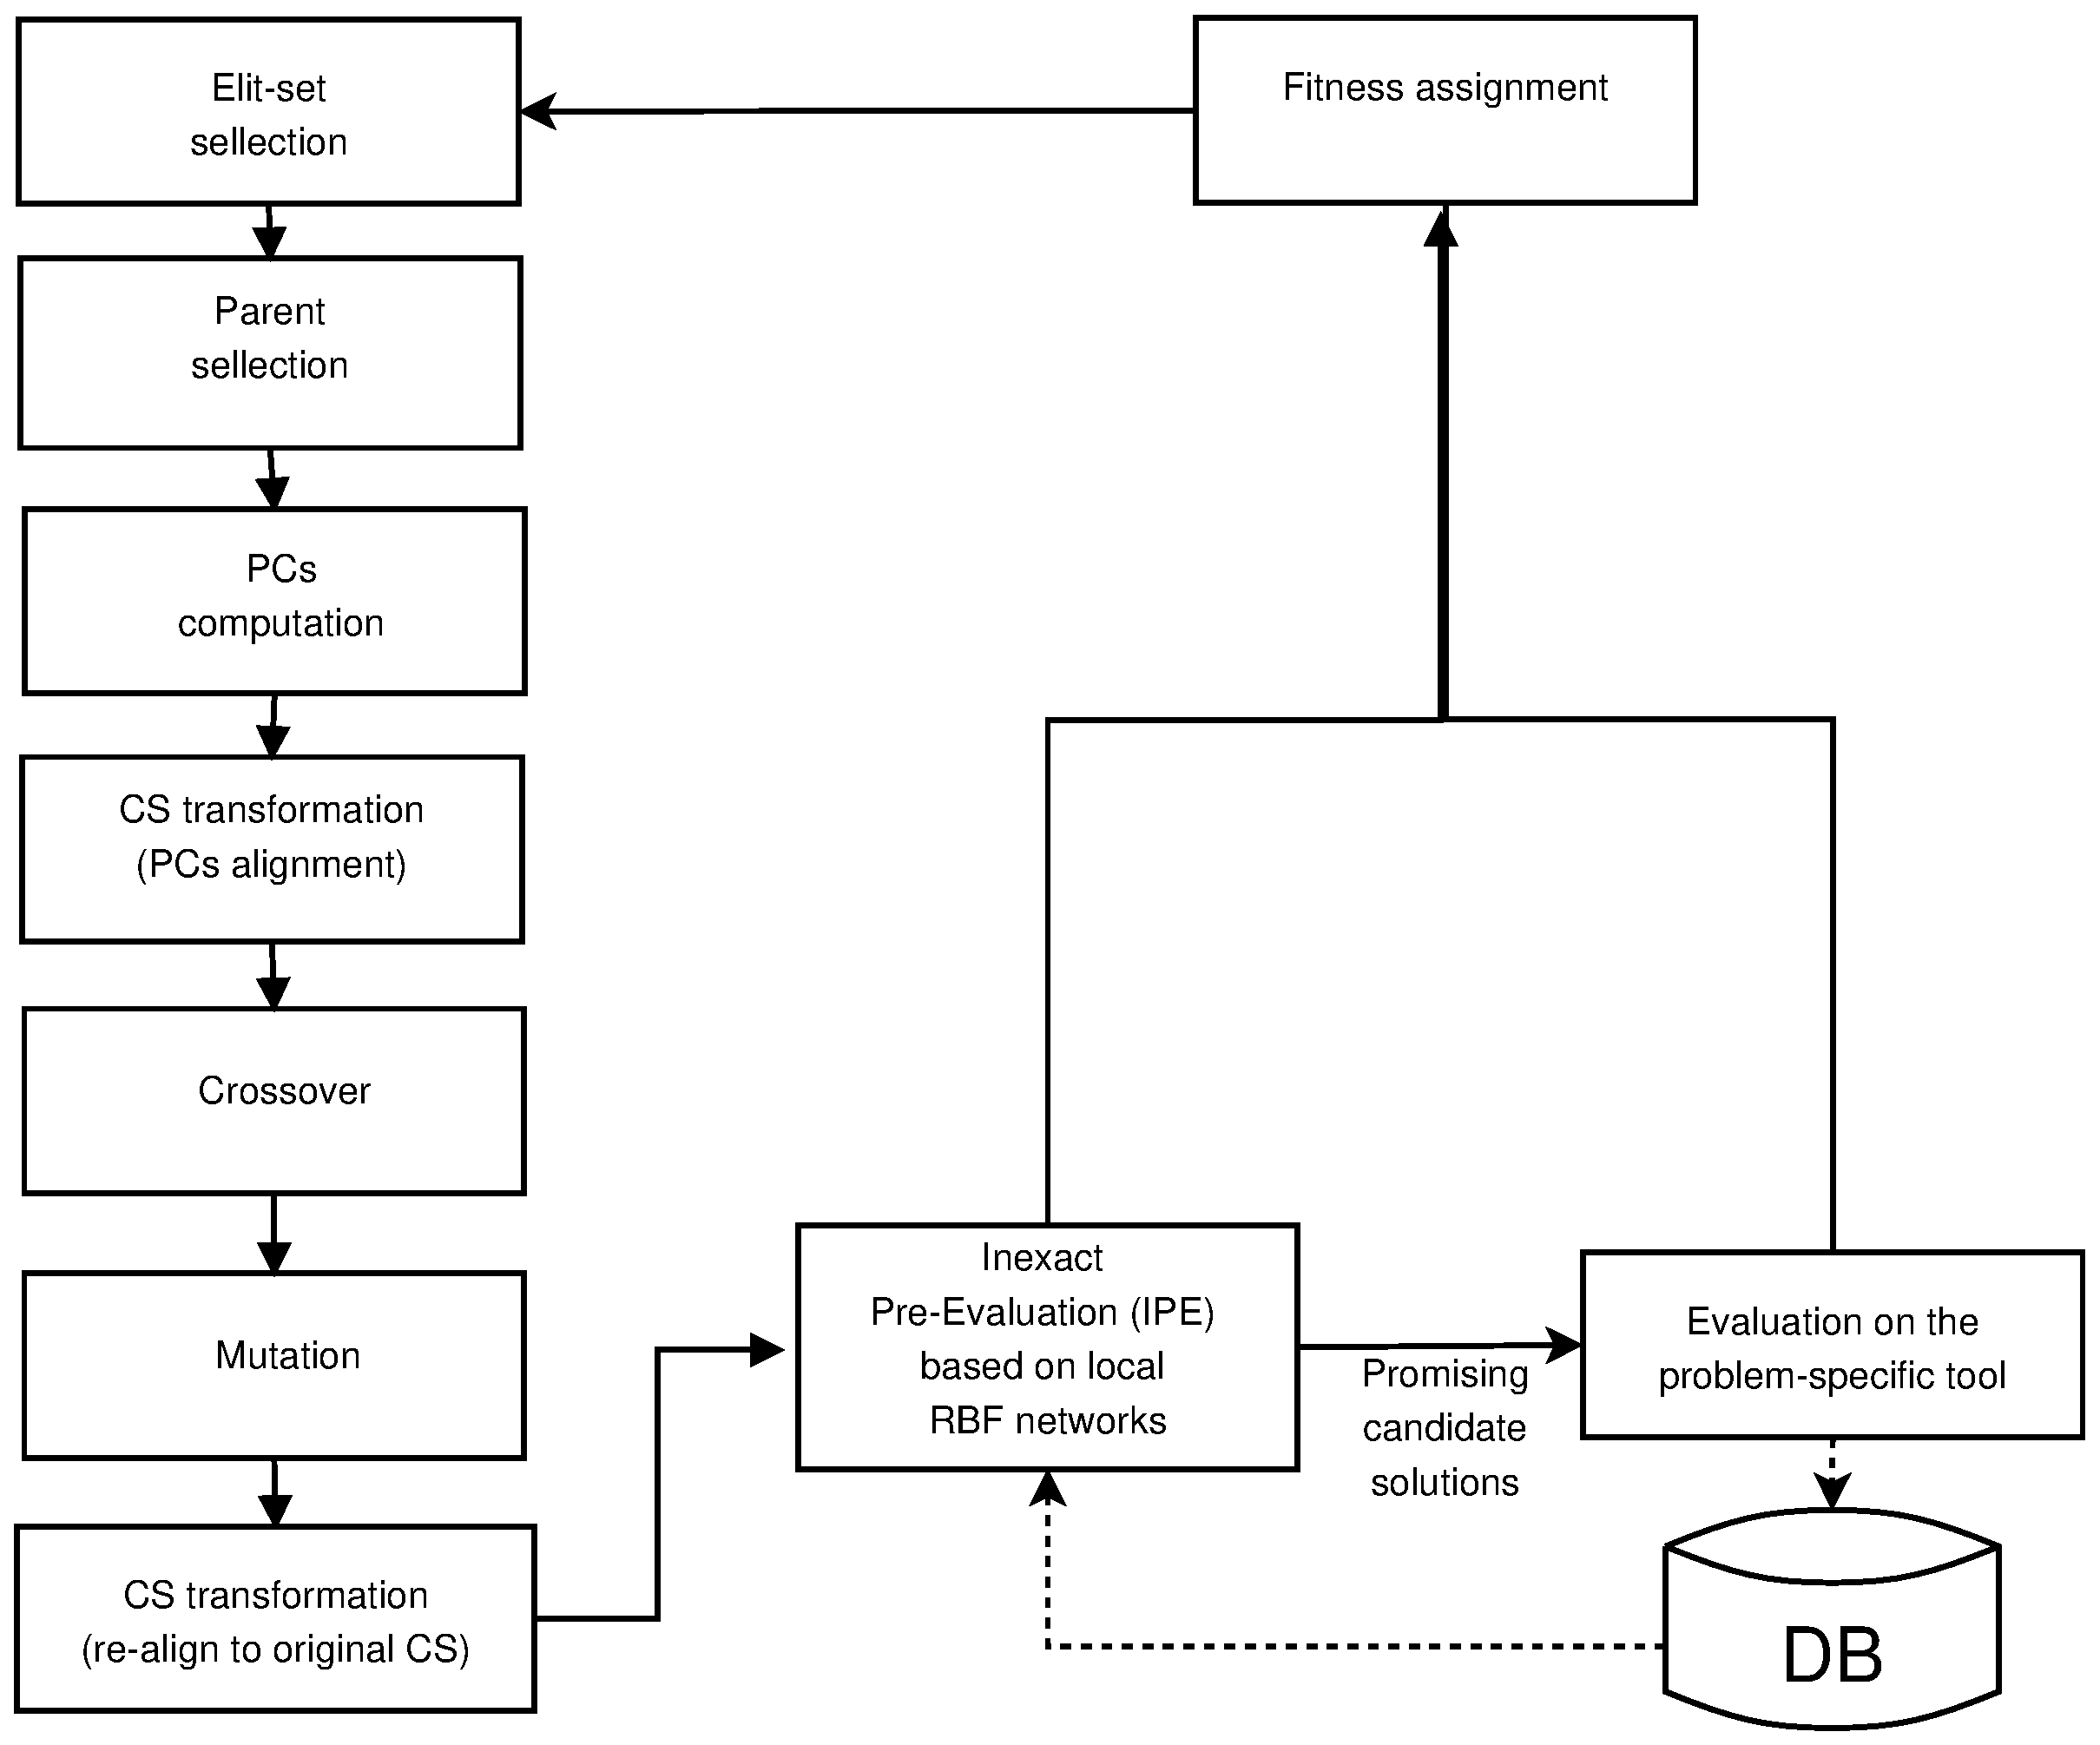
\includegraphics{MAEAPCA2.eps}}
%\end{minipage}
%\caption{Σχηματική απεικόνιση υποβοηθούμενου από μεταπρότυπα ΕΑ που κάνει χρίση τελεστών εξέλιξης υποβοηθούμενων από ΑσΚΣ (\english{MAEA(PCA)}).} 
%\label{MAEAPCA2}
%\end{figure}

\subsection{Πιστοποίηση εξελικτικών τελεστών υποβοηθού-μενων από ΑσΚΣ}
Το κέρδος απο τη χρήση των εξελικτικών τελεστών στις νέες μεταβλητές σχεδιασμού που ανέδειξε η ΑσΚΣ  ποσοτικοποιείται στα προβλήματα μαθηματικής ελαχιστοποίησης του 30Δ ελλειψοειδούς (σχέση \ref{ellipse}) και τις 30Δ πολυτροπικής συνάρτησης (σχέση \ref{mm}). 



\begin{figure}[h!]
%\begin{minipage}[b]{0.5\linewidth}
% \centering
% \resizebox*{7.5cm}{!}{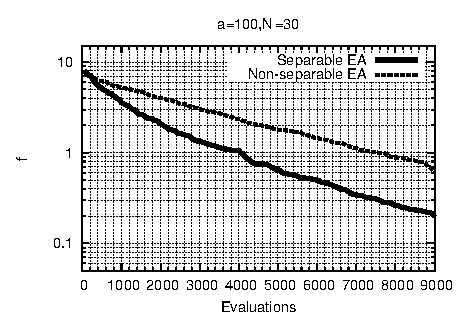
\includegraphics{100_30d.eps}}
%\end{minipage}
\begin{minipage}[b]{0.5\linewidth}
 \centering
 \resizebox*{7.5cm}{!}{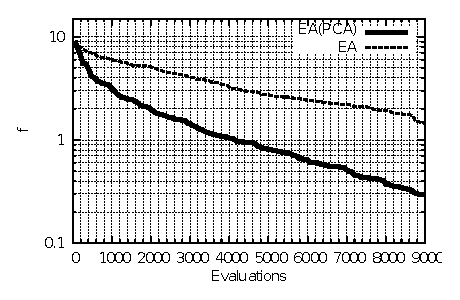
\includegraphics{1000_30d_pca.eps}}
\end{minipage}
\begin{minipage}[b]{0.5\linewidth}
 \centering
 \resizebox*{7.5cm}{!}{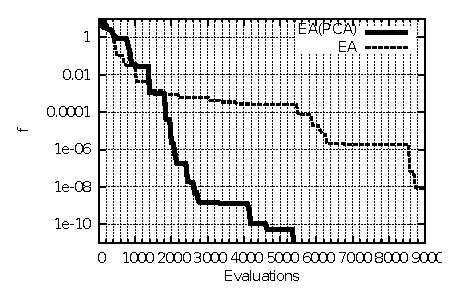
\includegraphics{30d_pca.eps}}
\end{minipage}
\caption{Πορείες σύγκλισης για το 30Δ ελλειψοειδές με αριθμό κατάστασης ($a\!=\!1000$) (αριστερά)  και την 30Δ συνάρτηση \ref{mm} (δεξιά). Η έντονη γραμμή παρουσιάζει την κατά πολύ βελτιωμένη σύγκλιση του ΕΑ στον οποίο οι εξελικτικοί τελεστές εφαρμόστηκαν στις εντοπιζόμενες από την ΑσΚΣ διαχωρίσιμες μεταβλητές σχεδιασμού.} 
\label{ellipse_t2_pca}
\end{figure} 

Οι πορείες σύγκλισης των ΕΑ και ΕΑ(\english{PCA}) για τις δύο αυτές συναρτήσεις παρουσιάζονται στο σχήμα \ref{ellipse_t2_pca}. Οι καμπύλες αποτελούν, και πάλι, τις μέσες τιμές των πορειών σύγκλισης που υπολογίσθηκαν τρέχοντας το ίδιο πρόβλημα $10$ φορές, κάθε φορά με διαφορετική αρχικοποίηση της γεννήτριας τυχαίων αριθμών.  Παρατηρείται ότι, και στα δύο προβλήματα, η χρήση των υποβοηθούμενων από την ΑσΚΣ τελεστών εξέλιξης υπερτερεί σημαντικά σε ταχύτητα και ανακτά ένα σημαντικό μέρος της μειωμένης απόδοσης των ΕΑ όταν αυτοί χρησιμοποιούνται για να λύσουν «κακώς τοποθετημένα» προβλήματα βελτιστοποίησης. 

\FloatBarrier
\section{Μεταπρότυπα Υποβοηθούμενα από ΑσΚΣ}
Η χρήση της ΑσΚΣ κατά τη διάρκεια εφαρμογής των τελεστών εξέλιξης δεν είναι η μόνη τεχνική που αποδείχθηκε ιδιαίτερα αποδοτική. Στην παρούσα διατριβή, προτείνεται επιπροσθέτως η χρήση των υπολογισθεισών, κατά την ΑσΚΣ, ιδιοτιμών ως μετρικών σημαντικότητας των κατευθύνσεων στο χώρο σχεδιασμού. Με τον τρόπο αυτό, η εκπαίδευση των μεταπροτύπων ενός ΜΑΕΑ πραγματοποιείται σε χώρο με αισθητά μειωμένη διάσταση. Τα μεταπρότυπα εκπαιδεύονται με μειωμένο αριθμό εισόδων, κρατώντας και χρησιμοποιώντας μόνο τις σημαντικότερες κατευθύνσεις στο χώρο σχεδιασμού που ανέδειξε η ΑσΚΣ και αποκόπτοντας τις λιγότερο σημαντικές. Η σημαντικότητα ορίζεται ως αντιστρόφως ανάλογη της ιδιοτιμής κάθε κατεύθυνσης στο χώρο σχεδιασμού.              



\begin{figure}
\begin{minipage}{0.48\textwidth}
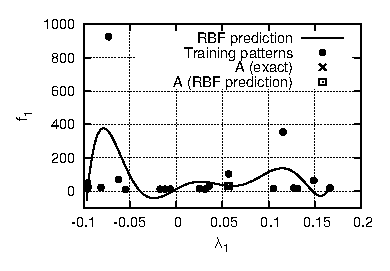
\includegraphics[scale=1.2]{IPE/f1_e1_b.eps}
\end{minipage}
\begin{minipage}{0.48\textwidth}
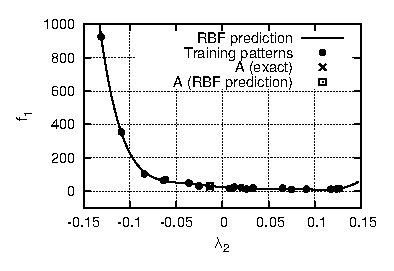
\includegraphics[scale=1.2]{IPE/f1_e2_b.eps}
\end{minipage}
\caption{ Εκτιμήσεις της τιμής της $f_1$ αν οι $\lambda_1$ (αριστερά) και $\lambda_2$ (δεξιά) χρησιμοποιηθούν, ξεχωριστά, ως είσοδοι του δικτύου \english{RBF}.}
\label{fig:f1e1e2}
\end{figure}

\begin{figure}
\begin{minipage}{0.48\textwidth}
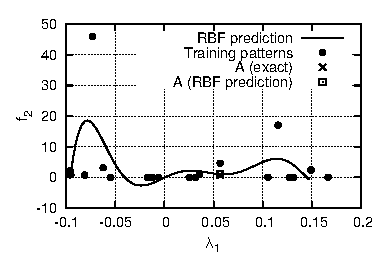
\includegraphics[scale=1.2]{IPE/f2_e1_b.eps}
\end{minipage}
\begin{minipage}{0.48\textwidth}
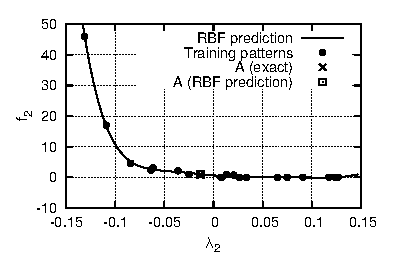
\includegraphics[scale=1.2]{IPE/f2_e2_b.eps}
\end{minipage}
\caption{Εκτιμήσεις της τιμής της $f_2$ αν οι $\lambda_1$ (αριστερά) και $\lambda_2$ (δεξιά) χρησιμοποιηθούν, ξεχωριστά, ως είσοδοι του δικτύου \english{RBF}.}
\label{fig:f2e1e2}
\end{figure}

%\begin{figure}[h!]
%\begin{minipage}[b]{0.5\linewidth}
% \centering
% \resizebox*{7.0cm}{!}{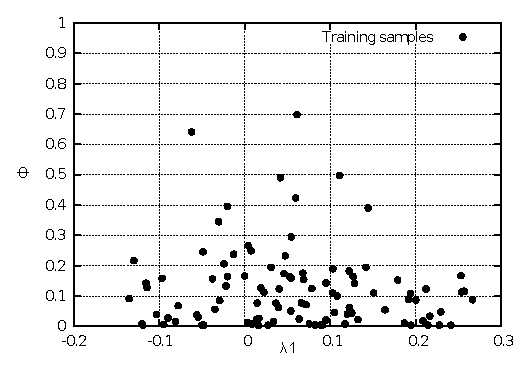
\includegraphics{1dANN_e1.eps}}
%\end{minipage}
%\begin{minipage}[b]{0.5\linewidth}
% \centering
% \resizebox*{7.0cm}{!}{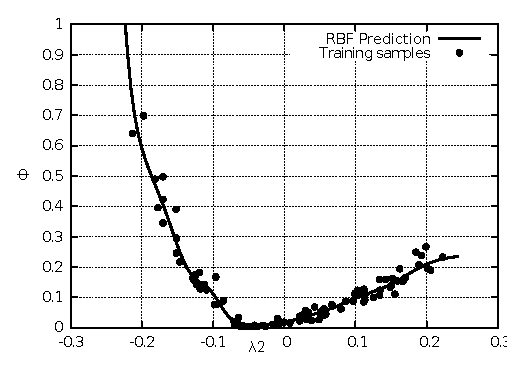
\includegraphics{1dANN_e2.eps}}
%\end{minipage}
%\caption{Εκτιμήσεις της τιμής της $\Phi$ από το μεταπρότυπο στο 2Δ πρόβλημα βελτιστοποίησης του σχήματος \ref{reco1}.  Πρότυπα εκπαίδευσης προβεβλημένα στο επίπεδο ($\Phi,\lambda_1$), όπου $\lambda_1$ η κατεύθυνση με τη μεγάλη ιδιοτιμή, βάσει της πραγματοποιηθείσας ΑσΚΣ (αριστερά). Πρότυπα εκπαίδευσης προβεβλημένα στο επίπεδο ($\Phi,\lambda_2$), όπου $\lambda_2$ η κατεύθυνση με τη μικρή ιδιοτιμή (δεξιά). Στην παρούσα διατριβή προτείνεται το μεταπρότυπo να εκπαιδευτεί μόνο στο  ($\Phi,\lambda_2$) επίπεδο, με το $\lambda_2$ δηλαδή ως τη μοναδική του είσοδο. Στο δεξιό σχήμα, με συνεχή γραμμή σχεδιάζεται η αναμενόμενη πρόβλεψη από το «σωστά» εκπαιδευμένο δίκτυο \english{RBF}. Στο αριστερό σχήμα, η αντίστοιχη καμπύλη αδυνατεί να παρακολουθήσει την ακατάστατη μορφή μορφή των αποκρίσεων και, για το λόγο αυτό, δεν σχεδιάζεται.} 
%\label{1dann}
%\end{figure}

Είναι εμφανές το πλεονέκτημα που επιφέρει η εκπαίδευση ενός μεταπροτύπου μόνο με τη συνιστώσα $\lambda_2$ (σχήμα  \ref{fig:f1e1e2} και \ref{fig:f2e1e2}), μιας και η κατά $\lambda_1$ συνιστώσα εισάγει ανεπιθύμητο θόρυβο και κάνει λιγότερο αξιόπιστη τη πρόβλεψη τόσο για την  $f_1$  όσο και για την $f_2$.   

\subsection{Πιστοποίηση του Μ($PCA$)ΑΕΑ($PCA$)}

Η συνδυασμένη χρήση της ΑσΚΣ για να τροποποιήσει τους τελεστές εξέλιξης αλλά και να βελτιώσει την αξιοπιστία των μεταπροτύπων, δηλαδή η τεχνική που συμβολίζεται ως Μ(\english{PCA})ΑΕΑ(\english{PCA}), πιστοποιείται στα προβλήματα ελαχιστοποίησης του 30Δ ελλειψοειδούς (σχέση \ref{ellipse}) και της 30Δ πολυτροπικής συνάρτησης (σχέση \ref{mm}). 


\begin{figure}[h!]
\begin{minipage}[b]{0.5\linewidth}
 \centering
 \resizebox*{7.5cm}{!}{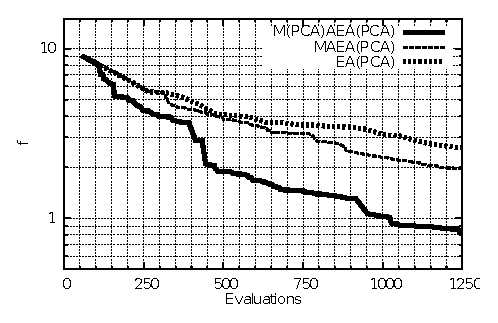
\includegraphics{1000_30d_pca_ipe.eps}}
\end{minipage}
\begin{minipage}[b]{0.5\linewidth}
 \centering
 \resizebox*{7.5cm}{!}{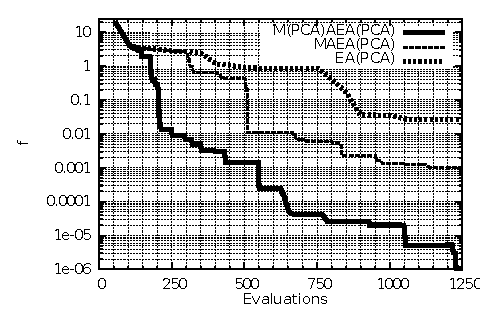
\includegraphics{30d_pca_ipe.eps}}
\end{minipage}
\caption{Μέσες καμπύλες σύγκλισης παραλλαγών των ΕΑ ή ΜΑΕΑ, που χρησιμοποιούν ΑσΚΣ, για το 30Δ ελλειψοειδές με  αριθμό κατάστασης $a=1000$ (αριστερά), και για την 30Δ συνάρτηση της σχέσης \ref{mm} (δεξιά).} 
\label{ellipse_t2_pca_ipe}
\end{figure} 
\pagebreak
Οι πορείες σύγκλισης των ΕΑ(\english{PCA}),    ΜΑΕΑ(\english{PCA}) και \linebreak Μ(\english{PCA})ΑΕΑ(\english{PCA}) για τα δύο αυτά προβλήματα παρουσιάζονται στο σχήμα \ref{ellipse_t2_pca_ipe}. Εκφράζουν και πάλι $10$ τρεξίματα βελτιστοποίησης με διαφορετική αρχικοποίηση της γεννήτριας τυχαίων αριθμών.  Παρατηρείται ότι η επιπρόσθετη χρήση υποβοηθούμενων απο ΑσΚΣ μεταπροτύπων επιφέρει επιπλέον μείωση του υπολογιστικού κόστους και στις δύο περιπτώσεις.


\section{Εφαρμογή: Σχεδιασμός 2Δ Πτερύγωσης Συμπιεστή}
Οι προτεινόμενες σε αυτό το κεφάλαιο μέθοδοι πιστοποιούνται, επίσης, στο σχεδιασμό-βελτιστοποίηση της αεροτομής μιας 2Δ πτερύγωσης συμπιεστή. Η πτερύγωση λειτουργεί σε $M_1=0.54$, $a_1=44^o$ και $Re=4\!\times\!10^5$ και στόχος είναι η ελαχιστοποίηση του συντελεστή των απωλειών ολικής πίεσης ($\omega$), σχέση \ref{omegaLosses}, υπό τους περιορισμούς ελάχιστου πάχους και ελάχιστης στροφής της ροής της ενότητας \ref{Drela1}. Χρησιμοποιείται το ίδιο λογισμικό αξιολόγησης. Η παραμετροποίηση της αεροτομής ορίζει συνολικά $27$ μεταβλητές σχεδιασμού.  

Πραγματοποιήθηκαν δύο διαδικασίες βελτιστοποίησης, η πρώτη με τον προϋπάρχοντα ΜΑΕΑ και η δεύτερη κάνοντας συνδυασμένη χρήση των δύο μεθόδων που προτάθηκαν σε αυτό το κεφάλαιο, δηλαδή τη μέθοδο Μ(\english{PCA})ΑΕΑ(\english{PCA}). 
   
Οι πορείες σύγκλισης για τις δύο αυτές διαδικασίες παρουσιάζονται στο σχήμα \ref{PCADrelaRes}, όπου είναι εμφανές το κέρδος που προκύπτει λόγω τόσο της ταχύτερης έναρξης της διαδικασίας ΠΠΑ όσο και της αποδοτικότερης εξέλιξης λόγω των προσαρμοσμένων τελεστών εξέλιξης. Περισσότερες πληροφορίες για τη ρύθμιση των παραμέτρων υπάρχουν στο πλήρες κείμενο της διατριβής.   
  

Η βέλτιστη αεροτομή, όπως αυτή προέκυψε από το συνδυασμό των προτεινόμενων μεθόδων παρουσιάζεται στο σχήμα \ref{PCADrelaRes2} και έχει απώλειες $\omega\!=\!0.01803$ και στροφή της ροής $\Delta a\!=\!30^o$ ενώ, παράλληλα, ικανοποιεί και όλους τους γεωμετρικούς περιορισμούς.  

\begin{figure}[h!]
\begin{minipage}[b]{1\linewidth}
 \centering
 \resizebox*{11cm}{!}{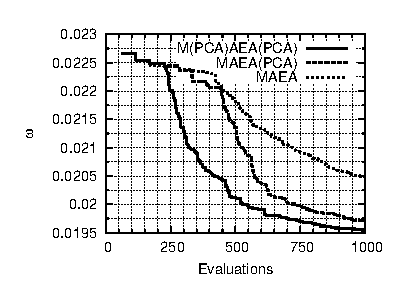
\includegraphics{CompConv_1.eps}}
\end{minipage}
\caption{Σχεδιασμός 2Δ πτερύγωσης συμπιεστή: Μέσες πορείες σύγκλισης από $10$ τρεξίματα των ΜΑΕΑ, ΜΑΕΑ(\english{PCA}) και  Μ(\english{PCA})ΑΕΑ(\english{PCA}). Ως κριτήριο τερματισμού τέθηκαν οι $1000$ κλήσεις του λογισμικού ΥΡΔ.} 
\label{PCADrelaRes}
\end{figure}


\begin{figure}[h!]
\begin{minipage}[b]{1\linewidth}
 \centering
 \resizebox*{14cm}{!}{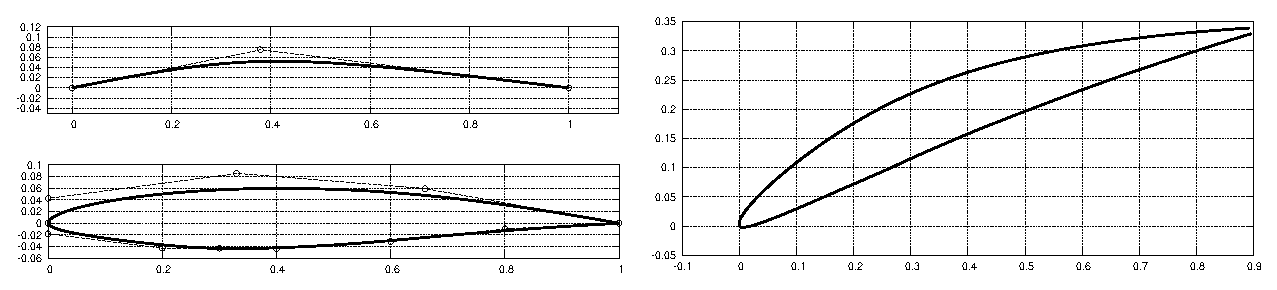
\includegraphics{ResD.eps}}
\end{minipage}
\caption{Σχεδιασμός 2Δ πτερύγωσης συμπιεστή: Η βέλτιστη αεροτομή, η οποία σχεδιάστηκε από το Μ(\english{PCA})ΑΕΑ(\english{PCA}). Αριστερά: Η μέση γραμμή και οι κατανομές πάχους για τις πλευρές υπερπίεσης και υποπίεσης, μαζί με τα πολύγωνα ελέγχου των πολυωνύμων \english{NURBS} που τις παρήγαγαν. Δεξιά: Η βέλτιστη αεροτομή, τοποθετημένη στην επιθυμητή γωνία κλίσης της πτερύγωσης. Η αεροτομή ικανοποιεί όλους τους τεθέντες περιορισμούς.} 
\label{PCADrelaRes2}
\end{figure}

%\begin{figure}[h!]
%\begin{minipage}[b]{1\linewidth}
% \centering
% \resizebox*{12cm}{!}{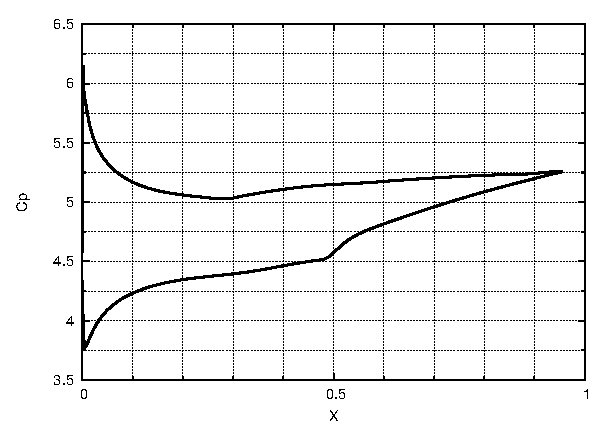
\includegraphics{Best_CP_PCA.eps}}
%\end{minipage}
%\caption{Σχεδιασμός 2Δ πτέρυγωσης συμπιεστή: Συντελεστής πίεσης $C_p$ για την βέλτιστη αεροτομή της εικόνας \ref{PCADrelaRes2}.} 
%\label{PCADrelaRes_cp}
%\end{figure}

% ---------------------------------------------------------------------------
% ----------------------- end of thesis sub-document ------------------------
% ---------------------------------------------------------------------------